\RequirePackage{etex}
\documentclass{beamer}
\usepackage[latin9]{inputenc}
\usepackage[ngerman]{babel}
\usepackage{amsmath}
\usepackage{listings}
\usepackage{color}
\usepackage{pictex}
\usepackage{tikz}
\usepackage{siunitx}

\title[CAN]{CAN - Controller Area Network}
\author{Dominik Eisele}
\institute[WSS]{Werner-Siemens-Schule}
\date{\today}
\subject{CAN}
\keywords{CAN, Controller Area Network}

\usetheme{Singapore}
\usecolortheme{rose}
\setbeamertemplate{navigation symbols}{}
\setbeamertemplate{footline}[frame number]
\beamersetuncovermixins{\opaqueness<1>{25}}{\opaqueness<2->{15}}

\definecolor{dkgreen}{rgb}{0,0.6,0}
\definecolor{gray}{rgb}{0.5,0.5,0.5}
\definecolor{mauve}{rgb}{0.58,0,0.82}

\lstset{language=C}
\lstset{numbers=left,
	numberstyle=\tiny,
	numbersep=5pt,
	breaklines=true,
	showstringspaces=false,
	frame=l ,
	xleftmargin=15pt,
	xrightmargin=15pt,
	basicstyle=\ttfamily\scriptsize,
	stepnumber=1,
	keywordstyle=\color{blue},		% keyword style
	commentstyle=\color{dkgreen},	% comment style
	stringstyle=\color{mauve}		% string literal style
}

%\AtBeginDocument{\addtobeamertemplate{block begin}{\setlength\abovedisplayskip{0pt}}}
%\AtBeginDocument{\addtobeamertemplate{block begin}{\setlength\abovedisplayshortskip{0pt}}}

\let\oldsqrt\sqrt
\def\sqrt{\mathpalette\DHLhksqrt}
\def\DHLhksqrt#1#2{\setbox0=\hbox{$#1\oldsqrt{#2\,}$}\dimen0=\ht0
\advance\dimen0-0.3\ht0
%0.3 ist das Ma� f�r die Hakenl�nge, relativ zum Inhalt der Wurzel
\setbox2=\hbox{\vrule height\ht0 depth -\dimen0}%
{\box0\lower0.4pt\box2}}

%\newif\ifsidebartheme
\sidebarthemetrue

\newdimen\contentheight
\newdimen\contentwidth
\newdimen\contentleft
\newdimen\contentbottom
\makeatletter
\newcommand*{\calculatespace}{%
\contentheight=\paperheight%
\ifx\beamer@frametitle\@empty%
    \setbox\@tempboxa=\box\voidb@x%
  \else%
    \setbox\@tempboxa=\vbox{%
      \vbox{}%
      {\parskip0pt\usebeamertemplate***{frametitle}}%
    }%
    \ifsidebartheme%
      \advance\contentheight by-1em%
    \fi%
  \fi%
\advance\contentheight by-\ht\@tempboxa%
\advance\contentheight by-\dp\@tempboxa%
\advance\contentheight by-\beamer@frametopskip%
\ifbeamer@plainframe%
\contentbottom=0pt%
\else%
\advance\contentheight by-\headheight%
\advance\contentheight by\headdp%
\advance\contentheight by-\footheight%
\advance\contentheight by4pt%
\contentbottom=\footheight%
\advance\contentbottom by-4pt%
\fi%
\contentwidth=\paperwidth%
\ifbeamer@plainframe%
\contentleft=0pt%
\else%
\advance\contentwidth by-\beamer@rightsidebar%
\advance\contentwidth by-\beamer@leftsidebar\relax%
\contentleft=\beamer@leftsidebar%
\fi%
}
\makeatother

\setcounter{tocdepth}{1}

\begin{document}

\begin{frame}
	\titlepage
\end{frame}

\begin{frame}{Inhalt}
	\tableofcontents
\end{frame}


\section{Allgemeine Informationen}
\subsection{Allgemeine Informationen-dots}

\begin{frame}{Geschichte}
	\begin{itemize}
		\item 1983 von Bosch als serielles Feldbussystem entwickelt
		\item Ziel war die Reduzierung der Kabelbauml�nge in Fahrzeugen
		\item Zertifiziert nach  ISO 11898-2 und  ISO 11898-3 (High- und Low-Speed CAN)
		\item CAN besitzt eine sehr sichere Daten�bertragung, welche Echtzeitanforderungen gerecht wird
	\end{itemize}
\end{frame}

\begin{frame}{Aufbau}
	\begin{figure}
		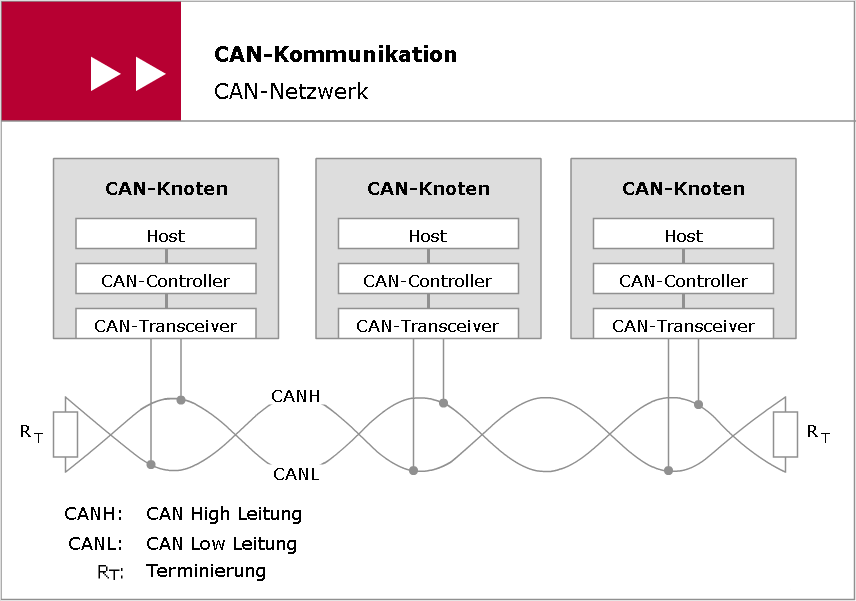
\includegraphics[height=0.7\textheight]{can_anschluss.PNG}
		\label{fig:aufbau}
	\end{figure}
\end{frame}


\begin{frame}{CAN-Buspegel}
	\begin{figure}
		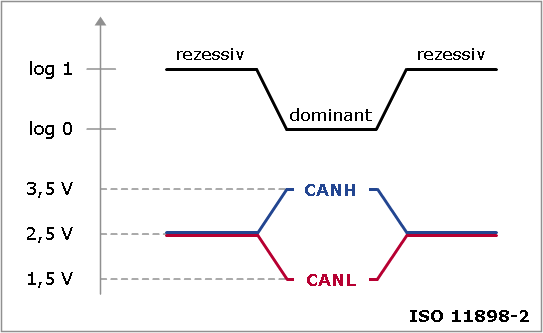
\includegraphics[scale=0.7]{can_highspeed.PNG}
		\label{fig:highspeed}
	\end{figure}
\end{frame}

\begin{frame}{CAN-Buspegel}
	\begin{figure}
		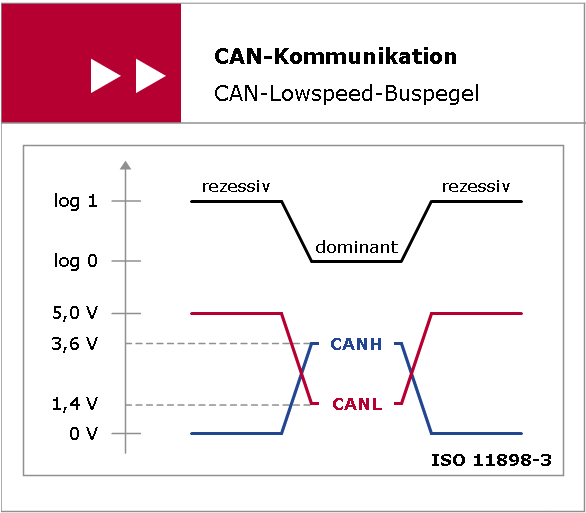
\includegraphics[scale=0.7]{can_lowspeed.PNG}
		\label{fig:lowspeed}
	\end{figure}
\end{frame}

\begin{frame}{Arbitrierung}
	\begin{itemize}
		\item CAN ist ein Multimasterbus, d.h. Teilnehmer m�ssen selbst entscheiden wann sie senden
		\item zum Einsatz kommt daher dass Carrier Sense Multiple Access/Collision Resolution (CSMA/CR) Verfahren
		\item wenn zwei Teilnehmer gleichzeitig senden kommt die bitweise Arbitrierung zum Einsatz
		\item bei der Arbitrierung werden die Identifier gleichzeitig gesendet und der Buspegel mit dem Sendepegel verglichen
		\item sendet ein Teilnehmer ein dominantes und ein anderer ein rezessives Bit wird der Buspegel dominant (logische 0)
	\end{itemize}
\end{frame}

\begin{frame}{Arbitrierung}
	\begin{figure}
		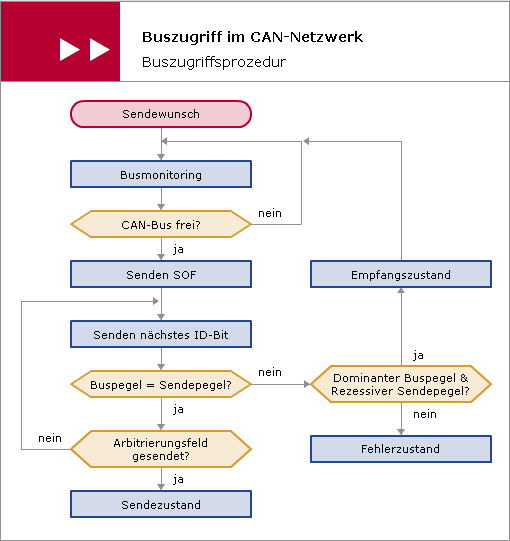
\includegraphics[scale=0.535]{buszugriff.PNG}
		\label{fig:buszugriff}
	\end{figure}
\end{frame}

\begin{frame}{Leitungsl�nge}
	\begin{figure}
		\begin{figure}[h!]
	\begin{tikzpicture}[xscale=0.8,yscale=0.6]
		% Achsen
		\draw[-] (0,0) -- (10,0) node[below] {\begin{tabular}{ll} \\  Leitungsl�nge in \si{\metre} \end{tabular}};
		\draw[-] (0,0) -- (0,9) node[below,left] {};
		\draw[-] (-1,4.5) -- (-1,4.5) node[left] {\begin{tabular}{l} k\\B\\i\\t\\s\\/\\s\end{tabular}};
		%Pfeile
		\draw[->] (0,0) -- (10,0);
		\draw[->] (0,0) -- (0,9);
		% Achsbeschriftung
		\foreach \x in {,1,...,9} \draw (\x,0.05) -- (\x,-0.05) node [below] {};
		\foreach \y in {1,...,8} \draw (0.1,\y) -- (-0.1,\y) node [left] {};		
		\draw (0,0) -- (0,0) node [below] {0};
		\draw (1,0) -- (1,0) node [below] {10};
		\draw (2,0) -- (2,0) node [below] {50};
		\draw (3,0) -- (3,0) node [below] {100};
		\draw (4,0) -- (4,0) node [below] {200};
		\draw (6,0) -- (6,0) node [below] {1000};
		\draw (9,0) -- (9,0) node [below] {10000};
		\draw (0,0) -- (0,0) node [left] {0};
		\draw (0,1) -- (0,1) node [left] {5};
		\draw (0,2) -- (0,2) node [left] {10};
		\draw (0,3) -- (0,3) node [left] {20};
		\draw (0,4) -- (0,4) node [left] {50};
		\draw (0,5) -- (0,5) node [left] {100};
		\draw (0,6) -- (0,6) node [left] {200};
		\draw (0,7) -- (0,7) node [left] {500};
		\draw (0,8) -- (0,8) node [left] {1000};
		\draw[smooth,samples=500,domain=0.0:8.24] plot(\x,{-0.062568 * \x^2 + -0.294511 * \x + 8.190863});
	\end{tikzpicture}
	\label{fig:Diagramm}
	\end{figure}
		\label{fig:leitunslaenge}
	\end{figure}
\end{frame}



\section{Protokoll}
\subsection{Protokoll-dots}
\begin{frame}{CAN-Frame}
	\begin{figure}
		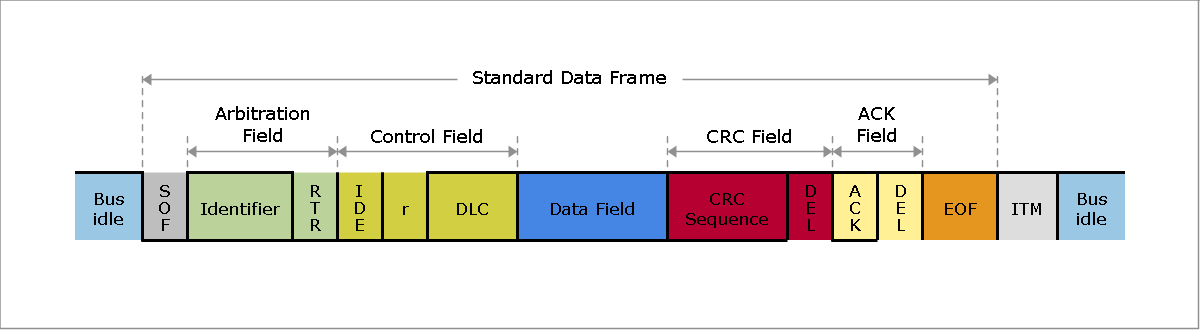
\includegraphics[width=\linewidth]{frame.PNG}
		\label{fig:frame}
	\end{figure}
\end{frame}

\begin{frame}{CAN-Frame}
	Start of Frame(SOF):
	\begin{figure}
		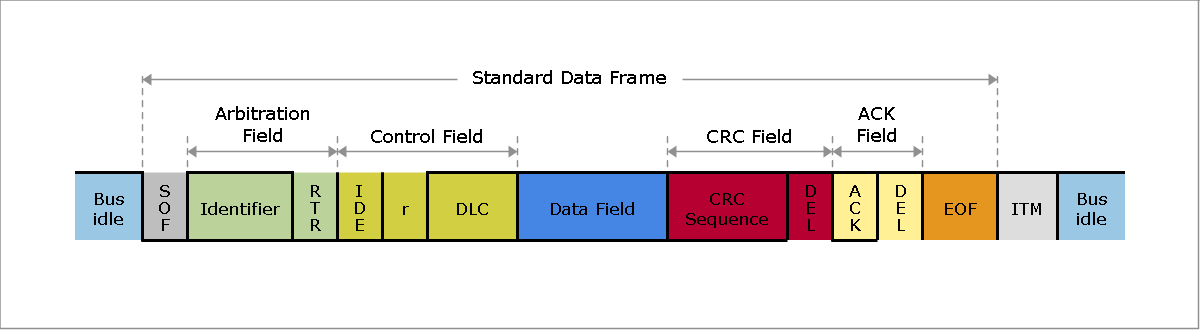
\includegraphics[width=\linewidth]{frame.PNG}
		\label{fig:frame}
	\end{figure}
	\begin{itemize}
		\item Start of Frame Bit ist ein dominantes Bit dass den Beginn einer Nachricht markiert
		\item wird zur zeitlichen Synchronisation der Knoten genutzt
	\end{itemize}
\end{frame}

\begin{frame}{CAN-Frame}
	Identifier:
	\begin{figure}
		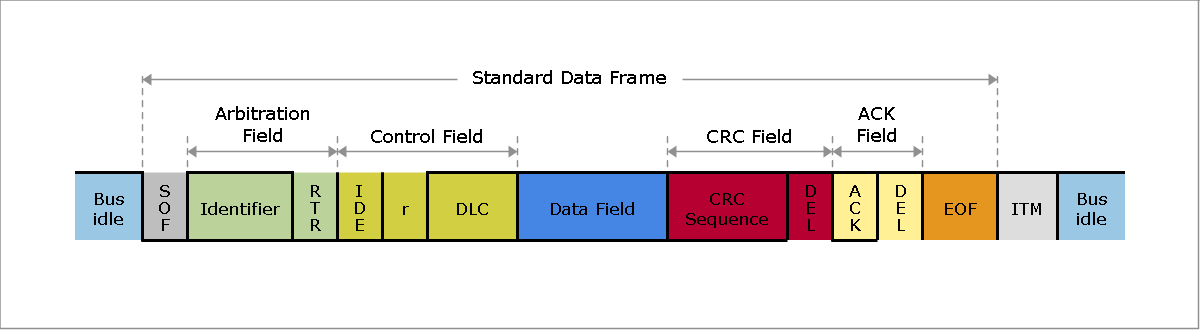
\includegraphics[width=\linewidth]{frame.PNG}
		\label{fig:frame}
	\end{figure}
	\begin{itemize}
		\item Identifier ist 11\ bit lang
		\item Extended Identifier hat 18 Zusatzbits
		\item Identifier markieren die Priorit�t der Nachricht
	\end{itemize}
\end{frame}

\begin{frame}{CAN-Frame}
	Remote Transmission Request (RTR):
	\begin{figure}
		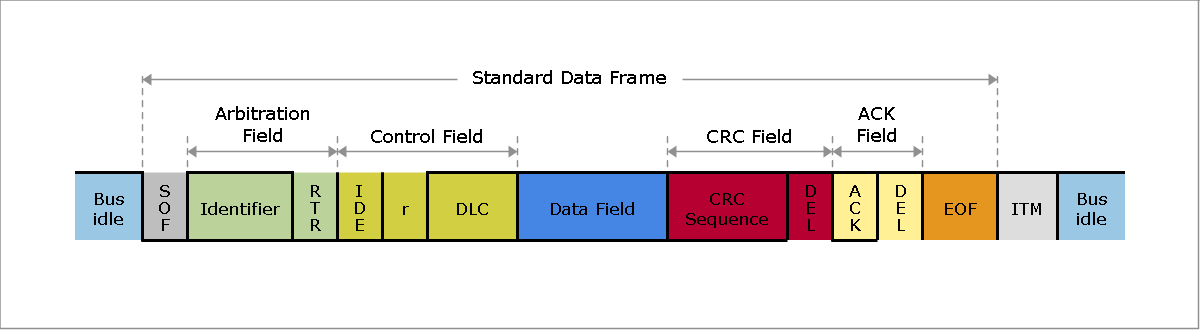
\includegraphics[width=\linewidth]{frame.PNG}
		\label{fig:frame}
	\end{figure}
	\begin{itemize}
		\item Remote Transmission Request Bit
		\item besitzt kein Data Field, sondern fordert Nachricht mit gleicher ID an wenn RTR rezessiv
	\end{itemize}
\end{frame}

\begin{frame}{CAN-Frame}
	Identifier Extension (IDE):
	\begin{figure}
		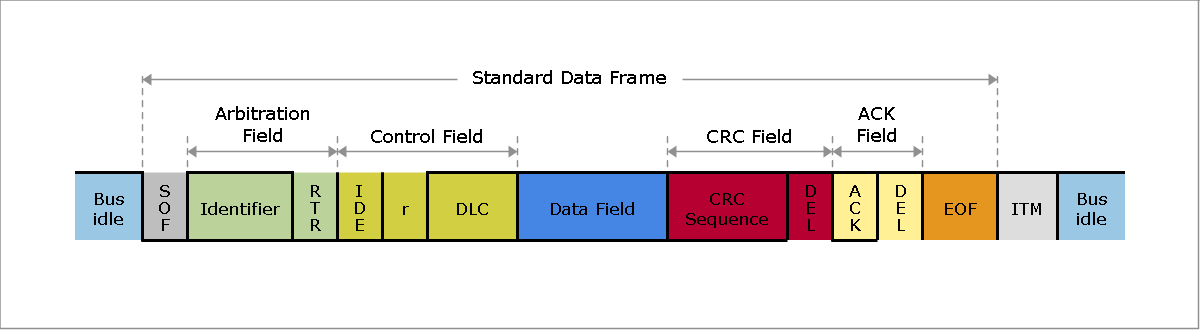
\includegraphics[width=\linewidth]{frame.PNG}
		\label{fig:frame}
	\end{figure}
	\begin{itemize}
		\item Identifier Extension Bit ist normal dominant
		\item wenn IDE rezessiv folgt erweiterter Identifier (18\ Bit)
	\end{itemize}
\end{frame}

\begin{frame}{CAN-Frame}
	Data Length Code (DLC):
	\begin{figure}
		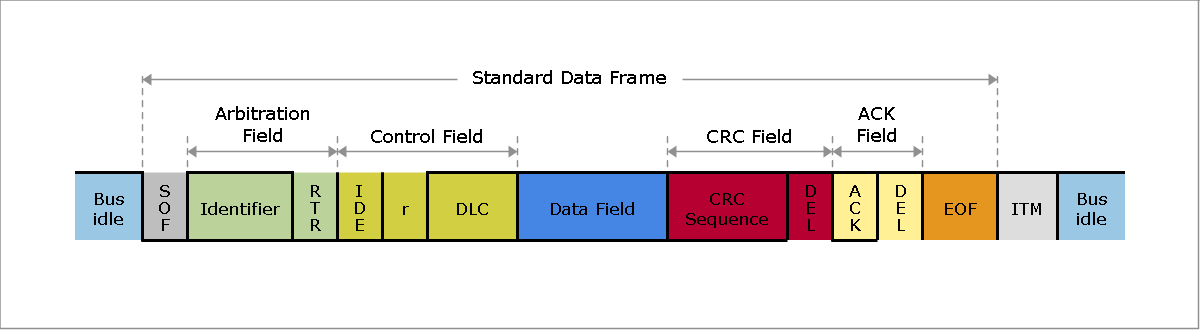
\includegraphics[width=\linewidth]{frame.PNG}
		\label{fig:frame}
	\end{figure}
	\begin{itemize}
		\item Data Length Code gibt die L�nge des Data Field an
		\item DLC sind 4\ Bit
		\item �bersteigt das DLC 8 ist die Datenl�nge totzdem 8 Byte, es k�nnen aber zus�tzliche Informationen �bermittelt werden
	\end{itemize}
\end{frame}

\begin{frame}{CAN-Frame}
	Data Field:
	\begin{figure}
		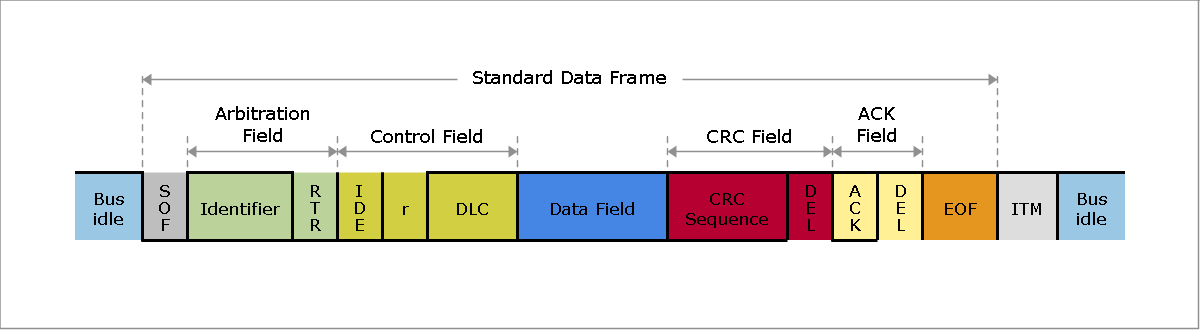
\includegraphics[width=\linewidth]{frame.PNG}
		\label{fig:frame}
	\end{figure}
	\begin{itemize}
		\item Data Field beinhaltet die Daten
		\item L�nge wird in DLC von 0 bis 8 Byte festgesetzt
	\end{itemize}
\end{frame}

\begin{frame}{CAN-Frame}
	Cyclic Redundancy Check (CLC):
	\begin{figure}
		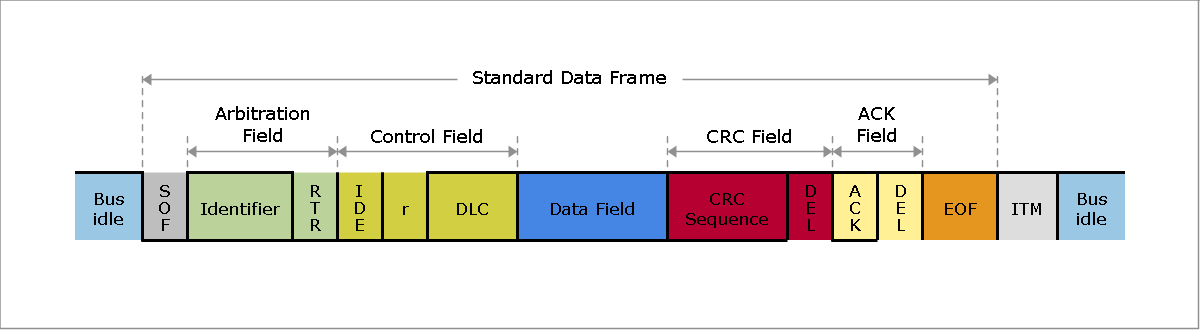
\includegraphics[width=\linewidth]{frame.PNG}
		\label{fig:frame}
	\end{figure}
	\begin{itemize}
		\item Cyclic Redundancy Check ist eine 15\ Bit lange Pr�fsequenz
		\item Mit der, in der Pr�fsequenz enthaltenen redundanten Information kann ein Empf�nger pr�fen, ob die Nachricht verf�lscht wurde.
		\item wird von rezessivem Delimiter-(DEL) Bit begrenzt
	\end{itemize}
\end{frame}

\begin{frame}{CAN-Frame}
	Acknowledge Field (ACK):
	\begin{figure}
		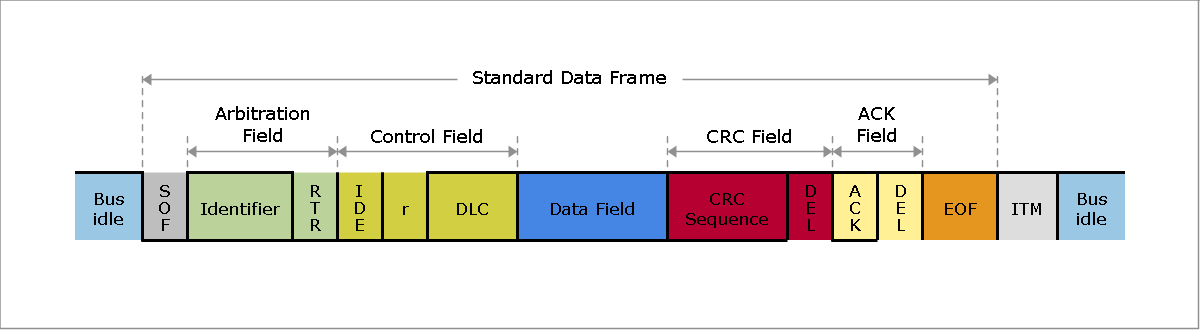
\includegraphics[width=\linewidth]{frame.PNG}
		\label{fig:frame}
	\end{figure}
	\begin{itemize}
		\item Acknowledge Field wird rezessiv gesendet, und bei korrektem Empfang von einem Empf�ner dominant �berschrieben
		\item wenn ACK rezessiv ist, wird die Nachricht erneut �bertragen
		\item wird bei einem Empf�nger ein Fehler erkannt, das ACK Bit ist aber gesetzt, so sendet er im Anschluss ein Error-Flag um die Nachricht erneut
		anzufordern, und die systemweite Datenkonsistenz zu wahren
	\end{itemize}
\end{frame}

\begin{frame}{CAN-Frame}
	Delimiter (DEL):
	\begin{figure}
		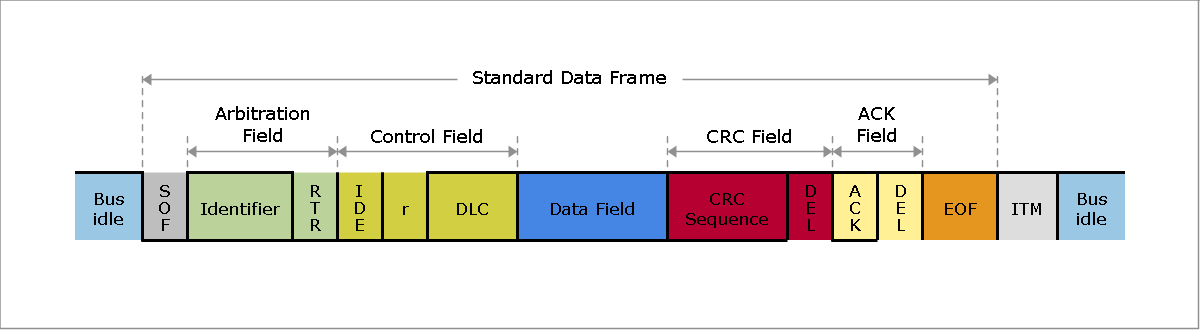
\includegraphics[width=\linewidth]{frame.PNG}
		\label{fig:frame}
	\end{figure}
	\begin{itemize}
		\item Delimiter begrenzt ACK-Field rezessiv
		\item wird bei lokalem Fehler eines Empf�ngers mit Error-Flag �berschrieben, sodass die Nachricht erneut gesendet wird
		\item dient der Unterscheidung zwischen Error-Flag und ACK-Field Ende
	\end{itemize}
\end{frame}

\begin{frame}{CAN-Frame}
	End of Frame (EOF):
	\begin{figure}
		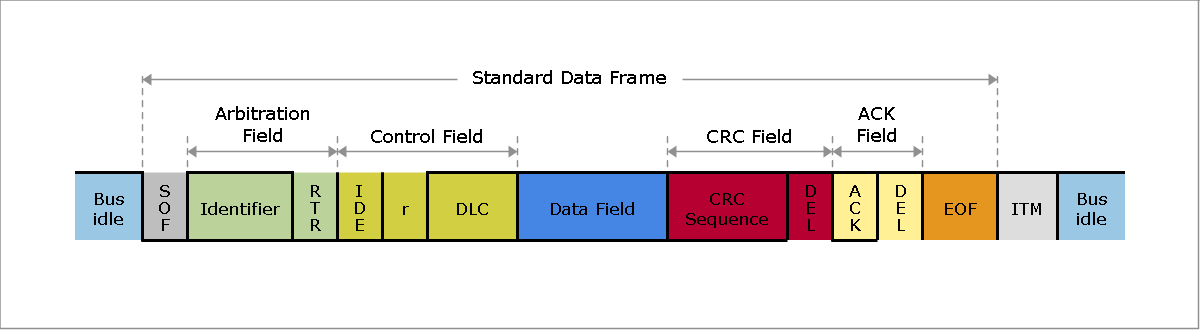
\includegraphics[width=\linewidth]{frame.PNG}
		\label{fig:frame}
	\end{figure}
	\begin{itemize}
		\item End of Frame Sequenz wird am Ende jeder Nachricht gesendet und besteht aus 8 rezessiven Bits
		\item lange Sequenz n�tig um Empf�ngern die M�glichkeit zu geben Fehler zu erkennen und zu Melden
	\end{itemize}
\end{frame}

\begin{frame}{Bit Stuffing}
	\begin{itemize}
		\item nach 5 gleichen Bits muss ein inverses Bit eingef�gt werden
		\item dient der Nachsynchronisierung der Busteilnehmer, da sie aufgrund ungenauen Taktzeiten der Oszillatoren auseinanderdriften k�nnen
		\item dient auserdem der Unterscheidung von Errorflags
		\item EOF ist vom Bitstuffing ausgenommen
		\item die Stopf-Bits werden vom Transmitter herausgefiltert
	\end{itemize}
\end{frame}

\begin{frame}{Fehlererkennung}
	\begin{itemize}
		\item Bit Monitoring
		\item Bit Stuffing
		\item Frame Check
		\item Acknowledgement Check
		\item Cyclic Redundancy Check
	\end{itemize}
\end{frame}

\begin{frame}{Fehlermeldung}
	\begin{itemize}
		\item jeder Empf�nger versucht einen Fehler zu erkennen und diesen umgehend zu dementieren
		\item Fehlermeldungen werden sofort nach erkennen des Fehlers gesendet
		\item ausgenommen hiervon ist das CRC-Feld um die ACK Funktion aufrecht zu erhalten
		\item Fehlermeldungen bestehen aus 6 gleichen Bits (rezessiv oder dominant)
		\item das Error-Flag zerst�rt den Bus Traffic
		\item wenn ein Fehler erkannt wird werden bei allen Empf�ngern die Nachrichten gel�scht, um eine systemweite Datenkonsistenz aufrecht zu erhalten
	\end{itemize}
\end{frame}

\begin{frame}{Bus Zust�nde}
	\begin{itemize}
		\item jeder Knoten hat zwei Error Counter (Transmit Error Counter und Error Counter)
		\item sendet ein Knoten ein Error Flag erh�ht sich der Counter um 8, empf�ngt er ein Flag erh�ht er sich um 1, bei korrektem Empfang wird er um 1 dekrementiert
		\item ist der Counter kleiner 127 sendet er als Error Flag 6 dominiante Bits, die den Bus �berschreiben und somit alle Nachrichten �berschreiben
		\item ist der Counter gr��er 127 werden 6 rezessive Bits gesendet, sodass der Bus nicht durchgehend gest�rt wird
		\item ist der Counter bei 255 angelangt darf der Teilnehmer nicht mehr am Bus teilnehmen
	\end{itemize}
\end{frame}







\section{Anwendungen}
\subsection{Anwendungen-dots}
\begin{frame}{Anwendungsbeispiele}
	\begin{itemize}
		\item Automobilindustrie
		\item Automatisierungstechnik
		\item Aufzugsanlagen
		\item Medizintechnik
		\item Flugzeugtechnik
		\item Raumfahrttechnik
		\item Schienenfahrzeuge
		\item Schiffbau
		\item Landwirtschaft
	\end{itemize}
\end{frame}


\section{Quellen}
\subsection{Quellen-dots}
\begin{frame}{Quellen}
	\begin{itemize}
		\item Konrad Etschberger - CAN Controller-Area-Network Grundlegen, Protokolle, Bausteine, Anwedungen
		\item Praxis Profiline - Controller-Area-Network CAN in Automation (CiA)
		\item elearning.vector.com (30.06.2016)
		\item kvaser.com (30.06.16)
		\item wikipedia.com (30.06.16)
	\end{itemize}
\end{frame}


\end{document}
